\ifx\allfiles\undefined

	% 如果有这一部分另外的package,在这里加上
	% 没有的话不需要
	
	\begin{document}
\else
\fi
    \chapter{整数规划}
    \section{整数规划问题与数学模型}
    \subsection{整数规划问题的定义}
    在前面的线性规划和运输规划问题中,最优解一般都是实数。但对于实际中的具体问题的解常常要求必须取整数,即称为整数解,
例如,问题答案是几个人、几台设备、几辆车等,无法用实数表达。因此,对于要求最优整数解的问题,就涉及到整数规划。
\begin{dfnbox}{整数规划}{amznotes}
    如果一个数学规划的\textcolor{red}{某些决策变量或全部决策变量}要求必须取\textcolor{red}{整数},则这样的问题称为\textbf{整数规划问题};
相应的模型称为\textbf{整数规划模型}。
\end{dfnbox}
\begin{itemize}
    \item \textbf{纯整数规划问题}:所有的决策变量都为\textcolor{red}{整数}的整数规划;
    \item \textbf{混合整数规划问题}:存在决策变量为\textcolor{red}{整数}的整数规划;
    \item \textbf{0-1规划}:所有的决策变量只能取\textcolor{red}{0或1}的整数规划;
\end{itemize}

\subsection{整数规划问题的数学模型}

\begin{thmbox}{一般形式的整数线性规划问题}{cool}
    \[
    \max(\min) \ z = \sum_{j=1}^{n} c_j x_j
    \]
    s.t.
    \[
    \begin{cases}
        \sum_{j=1}^{n} a_{ij} x_j \leq (\geq, =) b_i \,, & (i=1,2,\dots,m) \,, \\
        x_j \geq 0 \,, \quad x_j \text{ 为整数} & (j=1,2,\dots,n) \,.
    \end{cases}
    \]
\end{thmbox}

\begin{exbox}{\textbf{产品生产(纯整数规划问题)}}
    1\textbf{例}:某厂生产 $A_1$ 和 $A_2$ 两种产品,需要经过 $B_1$、$B_2$、$B_3$ 三道工序加工。单件工时和利润值以及各工序每月工时定额表 4.1。问工厂应如何安排生产才能使总利润最大?
    
    \begin{table}[H]
        \centering
        \label{tab:4.1}
        \renewcommand{\arraystretch}{1.5}
        \begin{tabular}{|c|c|c|c|c|}
            \hline
            & $B_1$ & $B_2$ & $B_3$ & 利润(元/件) \\ \hline
            $A_1$ & 0.3 & 0.2 & 0.3 & 25 \\ \hline
            $A_2$ & 0.7 & 0.1 & 0.5 & 40 \\ \hline
            工时定额(小时/月) & 250 & 100 & 150 & \\ \hline
        \end{tabular}
        \caption{工厂加工条件与利润}
    \end{table}
    
    \textbf{解:} 根据表 2-1 的最后一栏的利润数据,生产 $A_1$ 件、$A_2$ 件能获取的总利润为 $25x_1 + 40x_2$,因此,该问题的数学模型为:
    \begin{equation}
        \max \quad 25x_1 + 40x_2 \label{eq:Chapter4_obj_1}
    \end{equation}
    约束条件:
    \begin{align}
        0.3x_1 + 0.7x_2 &\leq 250 \,, \label{eq:c1} \\
        0.2x_1 + 0.1x_2 &\leq 100 \,, \label{eq:c2} \\
        0.2x_1 + 0.5x_2 &\leq 150 \,, \label{eq:c3} \\
        x_1 \geq 0 \,, \quad x_2 &\geq 0 \,. \label{eq:Chapter4_nonneg_1}
    \end{align}
    这是一个纯整数规划问题。
    
    \textbf{解}:设工厂每月生产 $A_1$ 产品 $x_1$ 件,$A_2$ 产品 $x_2$ 件。则按表 2-1 提供的条件数据,$A_1$ 产品 $x_1$ 件、$A_2$ 产品 $x_2$ 件加工需要的总利润为 $25x_1 + 40x_2$,因此,该问题的数学模型为:
    \begin{equation}
        \max \quad 25x_1 + 40x_2
    \end{equation}
    约束条件:
    \begin{align}
        0.3x_1 + 0.7x_2 &\leq 250 \,, \tag{$B_1$ 工序,工时限制} \\
        0.2x_1 + 0.1x_2 &\leq 100 \,, \tag{$B_2$ 工序,工时限制} \\
        0.2x_1 + 0.5x_2 &\leq 150 \,, \tag{$B_3$ 工序,工时限制} \\
        x_1 \geq 0 \,, \quad x_2 &\geq 0 \,. \tag{且只能整数}
    \end{align}
    另外,由于 $x_1$ 为 $A_1$ 的件数,因此 $x_1 \geq 0$ 且只能取整数;同理,$x_2 \geq 0$ 且只能取整数。
\end{exbox}


\begin{exbox}{\textbf{背包问题(0-1规划)}}
    1\textbf{例}:一个背包的总容积为 $V$,现要在 $n$ 种物品中选择。设物品 $j$ 的重量为 $w_j$,体积为 $v_j$,$j=1,2,\dots,n$。问如何选择,使得到的总价值最大,且总重量不超过 $V$,又使装的总重量最大。这一个题目有 $n$ 个约束情况,如装某类装箱,装箱,装车等。
    
    \textbf{解:} 设对于物品 $j$,变量
    \[
    x_j = \begin{cases} 
        1 & \text{物品 $j$ 被装入背包} \\ 
        0 & \text{物品 $j$ 不被装入背包}
    \end{cases} \quad j=1,2,\dots,n
    \]
    则所有被选择装物品的总体积为 $\sum_{j=1}^{n} v_j x_j$,总重量为 $\sum_{j=1}^{n} w_j x_j$,该问题的数学模型为:
    \begin{equation}
        \max \sum_{j=1}^{n} w_j x_j \label{eq:Chapter4_obj_2}
    \end{equation}
    约束条件:
    \begin{align}
        \sum_{j=1}^{n}  &v_j x_j\leq V \,, \label{eq:constraint} \\
        x_j &= 0, 1 \,, \quad j=1,2,\dots,n \,. \label{eq:binary}
    \end{align}
    这是一个 0-1 规划问题。
\end{exbox}


    \section{一般整数规划的求解方法—分枝定界法}
    为了解决整数规划问题,我们自然想到两种办法:
    \begin{itemize}
        \item 想到第二章提到的下料问题,可以用线性规划求解,结果四舍五入;
        \item 反正是整数,不妨穷举求解;
    \end{itemize}
    显然第一个方法不够靠谱,第二个方法效率太低。\\
    \begin{exbox}{\textbf{第一个方法不靠谱的原因}}
    1例如, 考虑如下整数规划问题:
    \begin{align}
        \max \ 3x_{1} &+ 13x_{2} \\
        \text{s.t.} \quad 2x_{1} + 9x_{2} &\leq 40 \\
        11x_{1} - 8x_{2} &\leq 82 \\
        x_{1} \geq 0, \quad x_{2} &\geq 0 \quad \text{且取整数}
    \end{align}
    画出可行域如下所示\footnote{图中可以看到,浮点数最优解 B四周的四个整数点都不在可行域内,四舍五入的结果是错误的。反而整数最优解在C点。}:
    \begin{figure}[H]
        \centering
        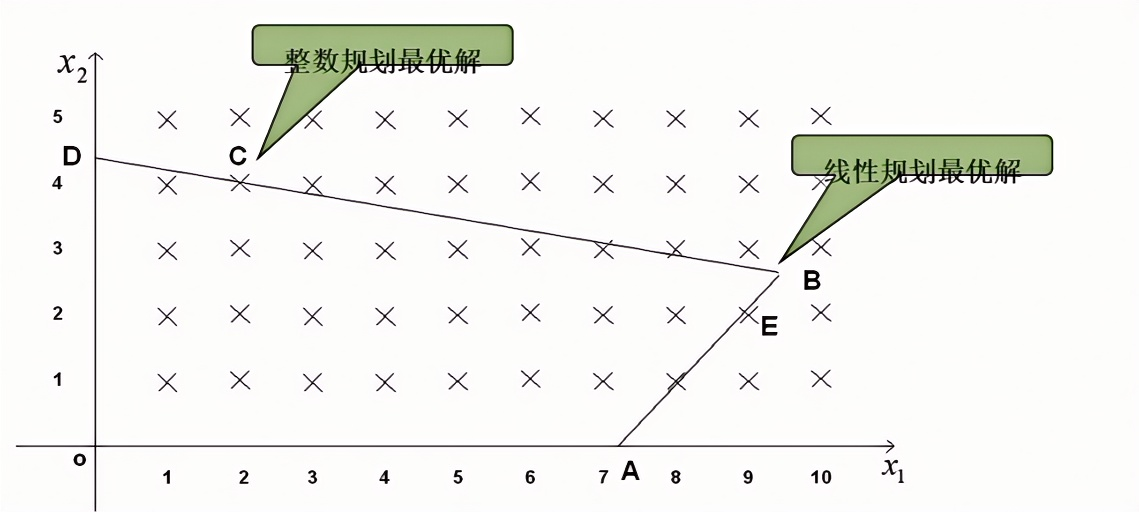
\includegraphics[width=0.8\textwidth]{./image/8.png}
        \caption{整数规划的四舍五入求解}
        \label{fig:Chapter4_Temporary_Pavilion_1}
    \end{figure}
    \end{exbox}

    目前,常用的求解整数规划的方法是分枝定界法和割平面法。作为一种最基本的方法,下面介绍分枝定界法。
    \begin{notebox}{\textbf{分枝定界法}}
        \label{分枝定界法}
        \\
        \begin{enumerate}
            \item 设有最大化的整数规划问题A,与它相应的线性规划问题(即在整数规划中去掉了决策变量的整数取值要求)为B,设二者的最优值分别为$z_A^*$和$z_B^*$;
            \item 从解问题B开始,若B的最优解符合A中的整数条件,\textcolor{red}{则A的最优解即为B的最优解},结束;
            \item 若B的最优解不符合A的整数条件,则B的最优解对应的最优值$z_B^*$一定是\textcolor{red}{A的最优值$z_A^*$的上界},记为$\overline{z}$ ,而A的某一\textcolor{red}{任一可行解}(即任意一个整数解)的目标函数值将是一个下界$\underline{z}$。此时$\underline{z}\leq z_A^* \leq \overline{z}$,称为\textbf{定界};
            \item 分枝定界法即不断将B的可行域分成子区域(称为\textbf{分枝}),并在每个子区域中确定A的\textcolor{red}{上界$\overline{z}$和下界$\underline{z}$}的方法,逐步夹逼,直到找到A的最优解为止;
        \end{enumerate}
    \end{notebox}

    \begin{figure}[H]
        \centering
        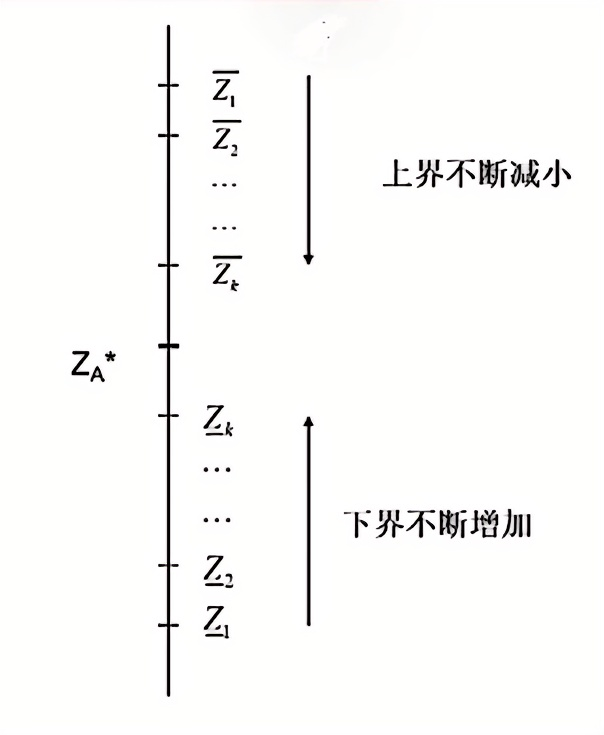
\includegraphics[width=0.5\textwidth]{./image/9.png}
        \caption{分枝定界法}
        \label{fig:Chapter4_Temporary_Pavilion_2}
    \end{figure}
    \begin{exbox}{\textbf{分枝定界法}}
        1\textbf{例:}\ 考虑如下整数规划问题:
        \begin{align}
            \max \ 40x_{1} &+ 90x_{2} \\
            \text{s.t.} \quad 9x_{1} + 7x_{2} &\leq 56 \\
            7x_{1} + 20x_{2} &\leq 70 \\
            x_{1} \geq 0, \quad x_{2} &\geq 0 \quad \text{且取整数}
        \end{align}
        \textbf{解:}\ 记上述原问题为A。先考虑A中去掉整数约束条件后的线性规划问题B.
        \\
        对问题B进行第二章中所学到的线性规划分析,可以找到最优解,依照\hyperref[分枝定界法]{分枝定界法},发现B的最优解并非整数,说明\textcolor{red}{需要继续迭代},因此我们记B的最优解对应的最优值$z_B^*=356$作为一个上界,并任意找一个A的可行解如原点,得到下限$\underline{z}=0$,此时$\underline{z}\leq z_A^* \leq \overline{z}$,即$0\leq z_A^* \leq 356$。如下图所示:\\
        \begin{figure}[H]
            \centering
            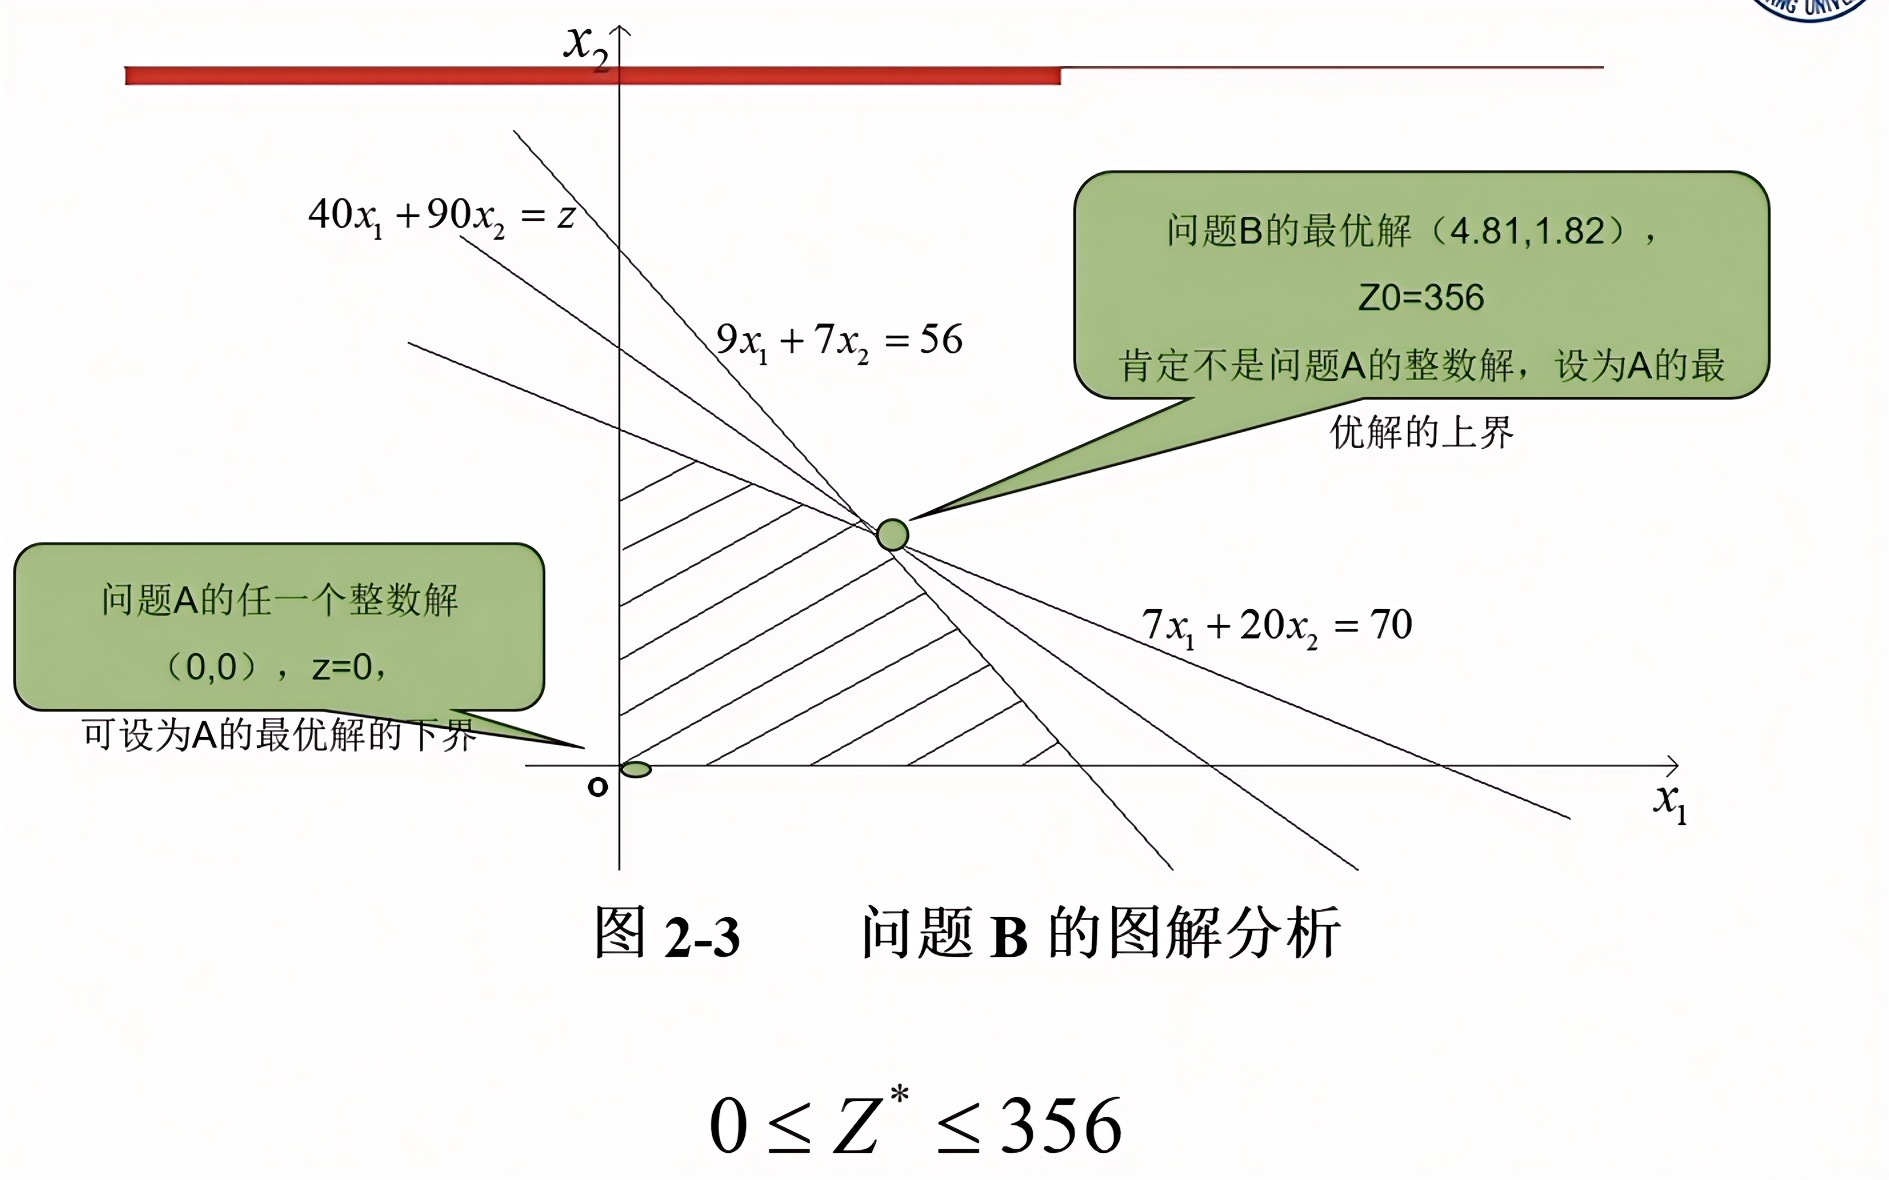
\includegraphics[width=0.8\textwidth]{./image/11.png}
            \caption{问题B的图解分析}
            \label{fig:Chapter4_Temporary_Pavilion_3}
        \end{figure}
        在问题 B 中最优解为 \( {x}_{1} = {4.81} \) ,于是对 B 通过增加两个
        约束条件 \( {x}_{1} \leq  4 \) 和 \( {x}_{1} \geq  5 \) 可将 B 分解为两个子问题 \( {B}_{1} \) 和 \( {B}_{2} \) ,即将 B
        的可行域在 \( {x}_{1} = {4.81} \) 前后分割为两个子可行域(称为分枝), 中间因为不满足整数条件而舍弃,如下图所示:
        \begin{figure}[H]
            \centering
            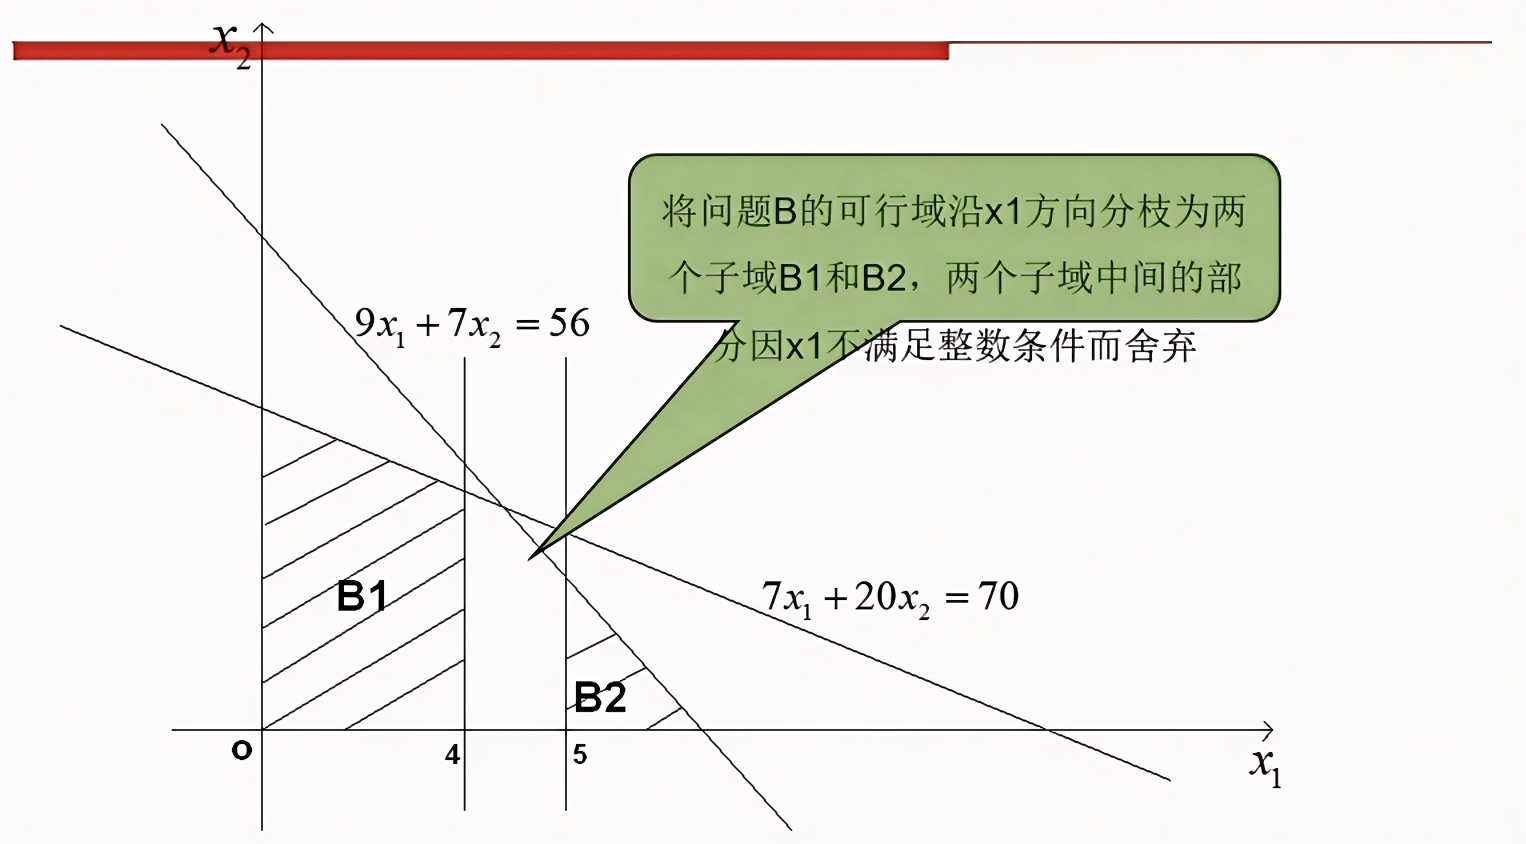
\includegraphics[width=0.8\textwidth]{./image/10.png}
            \caption{问题B的分枝}
            \label{fig:Chapter4_Temporary_Pavilion_4}
        \end{figure}
        对应的 $\text{B}_1$ 和 $\text{B}_2$ 分别为:

        \textbf{问题 B1}:
        
        \begin{align*}
        \max \quad & 40x_1 + 90x_2 \\
        \text{s.t.} \quad & 9x_1 + 7x_2 \leq 56 \\
        & 7x_1 + 20x_2 \leq 70 \\
        & 0 \leq x_1 \leq 4 \\
        & x_2 \geq 0
        \end{align*}
        
        \textbf{问题 B2}:
        
        \begin{align*}
        \max \quad & 40x_1 + 90x_2 \\
        \text{s.t.} \quad & 9x_1 + 7x_2 \leq 56 \\
        & 7x_1 + 20x_2 \leq 70 \\
        & x_1 \leq 5 \\
        & x_2 \geq 0
        \end{align*}
        \textbf{这样,我们进行第一次迭代。}\\
        在两个区域内分别线性规划求解,如下图所示,两处最优解仍然不都是整数,说明\textcolor{red}{需要继续迭代}。B1区域的最优值是$z_{B1}^* = 349$,B2区域的最优值是$z_{B2}^* = 341$,取较大的那个,因此新的上限是$z_{B1}^* = 349$,下限依然是$z_{B}^* = 0$(注意下界此处不是不可以动,而是我们懒得去动),所以我们将上限从原来的356调整为349,此时$0\leq z_A^* \leq 349$。\\
        \begin{figure}[H]
            \centering
            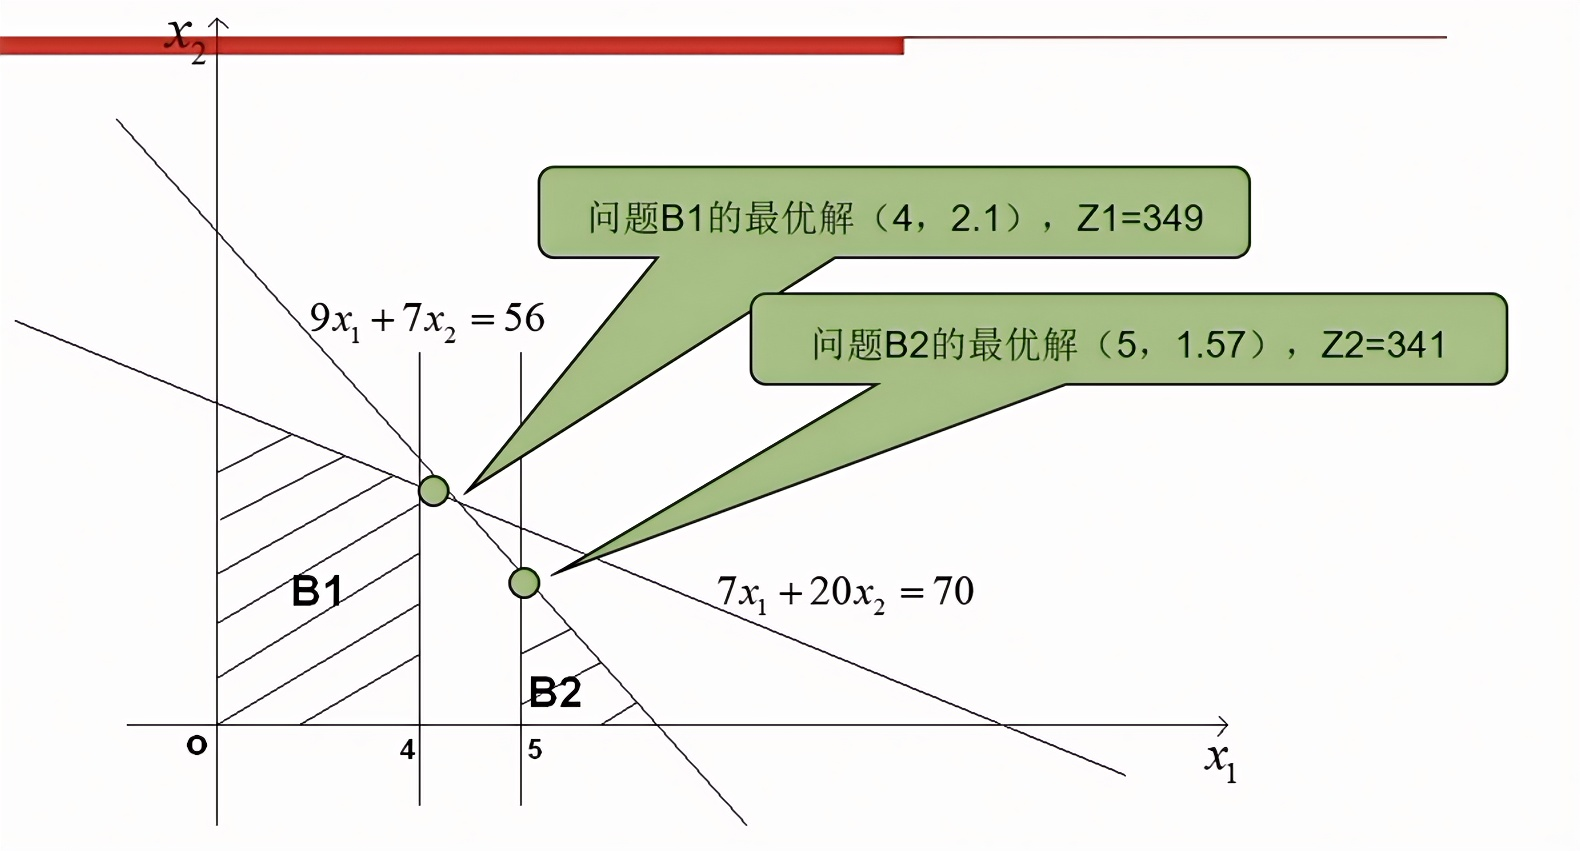
\includegraphics[width=0.8\textwidth]{./image/12.png}
            \caption{第一次迭代}
            \label{fig:Chapter4_Temporary_Pavilion_4}
        \end{figure}
        继续对 \( \text{B}_{1} \) 和 \( \text{B}_{2} \) 进行分解。因 \( {z}_{1} > {z}_{2} \) ,故先分解 \( \text{B}_{1} \) 为两枝。此
        次沿 \( {x}_{2} \) 方向分解,增加约束条件 \( {x}_{2} \leq  2 \) ,称为问题 \( \text{B}_{3} \) ; 增加约束
        条件 \( {x}_{2} \geq  3 \) ,称为问题 \( \text{B}_{4} \) 。在图 2-4 中舍去 \( {x}_{2} > 2 \) 与 \( {x}_{2} < 3 \) 之间的
        可行域。\\
        \textbf{这样,我们进行第二次迭代。}\\
        在两个区域内分别线性规划求解,可以发现B3的最优点仍是顶点,恰好是整数$(4,2)$\footnote{读者不妨想到此事并非偶然。事实上,由于我们的切割线总是$x_1=a$或$x_2=b$,总是能割出一个区域为矩形,顶点就是整数解},最优值是$z_{B3}^* = 340$,
        这个数可能是上界(即整数里最优的),也可能不是,但至少一定是整数中的一员,所以肯定可以作为下界\footnote{读者可能会感到疑问,之前方法里不是说算到是整数解就应该停止迭代作为最优解了吗?为什么还要继续算呢?读者不妨想到,这个整数解确实是最优解,但是不是问题A的最优解,而是问题B3对应的A3的最优解,所以仍需要证明其他区域内没有比这个更大或者有更大的最优值了}。而B4的最优值都比不上我们新的下界了,那B4就失去了意义,不必再分割了;同理B3也不需要再分割了,最大值是下限,再求B3也没有比340更大的整数解了;但是B2有必要继续去做切割。如下图所示:
        \begin{figure}[H]
            \centering
            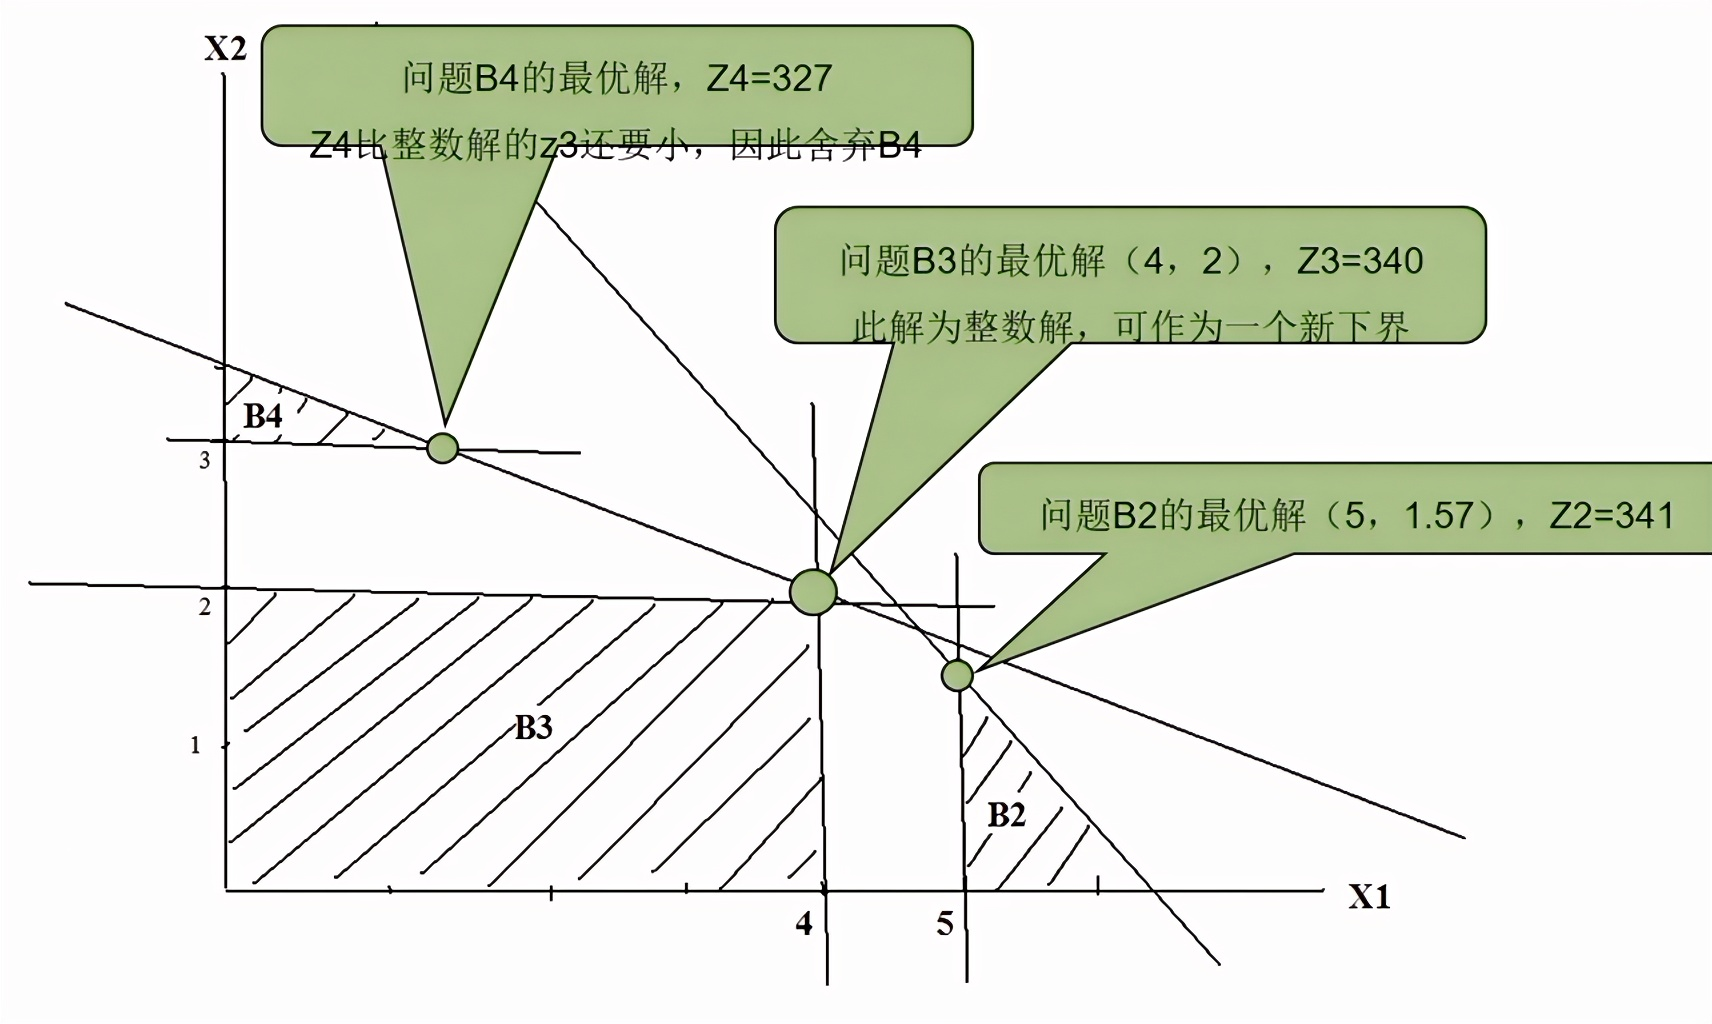
\includegraphics[width=0.8\textwidth]{./image/13.png}
            \caption{第二次迭代}
            \label{fig:Chapter4_Temporary_Pavilion_4}
        \end{figure}
        既然 $\text{B}_1$ 中已不存在上限,于是分解 $\text{B}_2$ 得以下问题:\\
        \textbf{问题 B5}:
        \begin{align*}
        \max \quad & 40x_1 + 90x_2 \\
        \text{s.t.} \quad & 9x_1 + 7x_2 \leq 56 \\
        & 7x_1 + 20x_2 \leq 70 \\
        & 5 \leq x_1 \\
        & 0 \leq x_2 \leq 1
        \end{align*}
        \textbf{问题 B6}:
        \begin{align*}
        \max \quad & 40x_1 + 90x_2 \\
        \text{s.t.} \quad & 9x_1 + 7x_2 \leq 56 \\
        & 7x_1 + 20x_2 \leq 70 \\
        & 5 \leq x_1 \\
        & 2 \leq x_2
        \end{align*}
        \textbf{这样,我们进行第三次迭代。}\\
        在两个区域内分别线性规划求解,可以发现B6没有可行解,故B6不再需要分割;B5的最优解$z_{B5}^* = 308$小于下限,故B5不再需要分割;因此,可以得出结论,最优解就是$z_{B3}^* = 340$如下图所示:
        \begin{figure}[H]
            \centering
            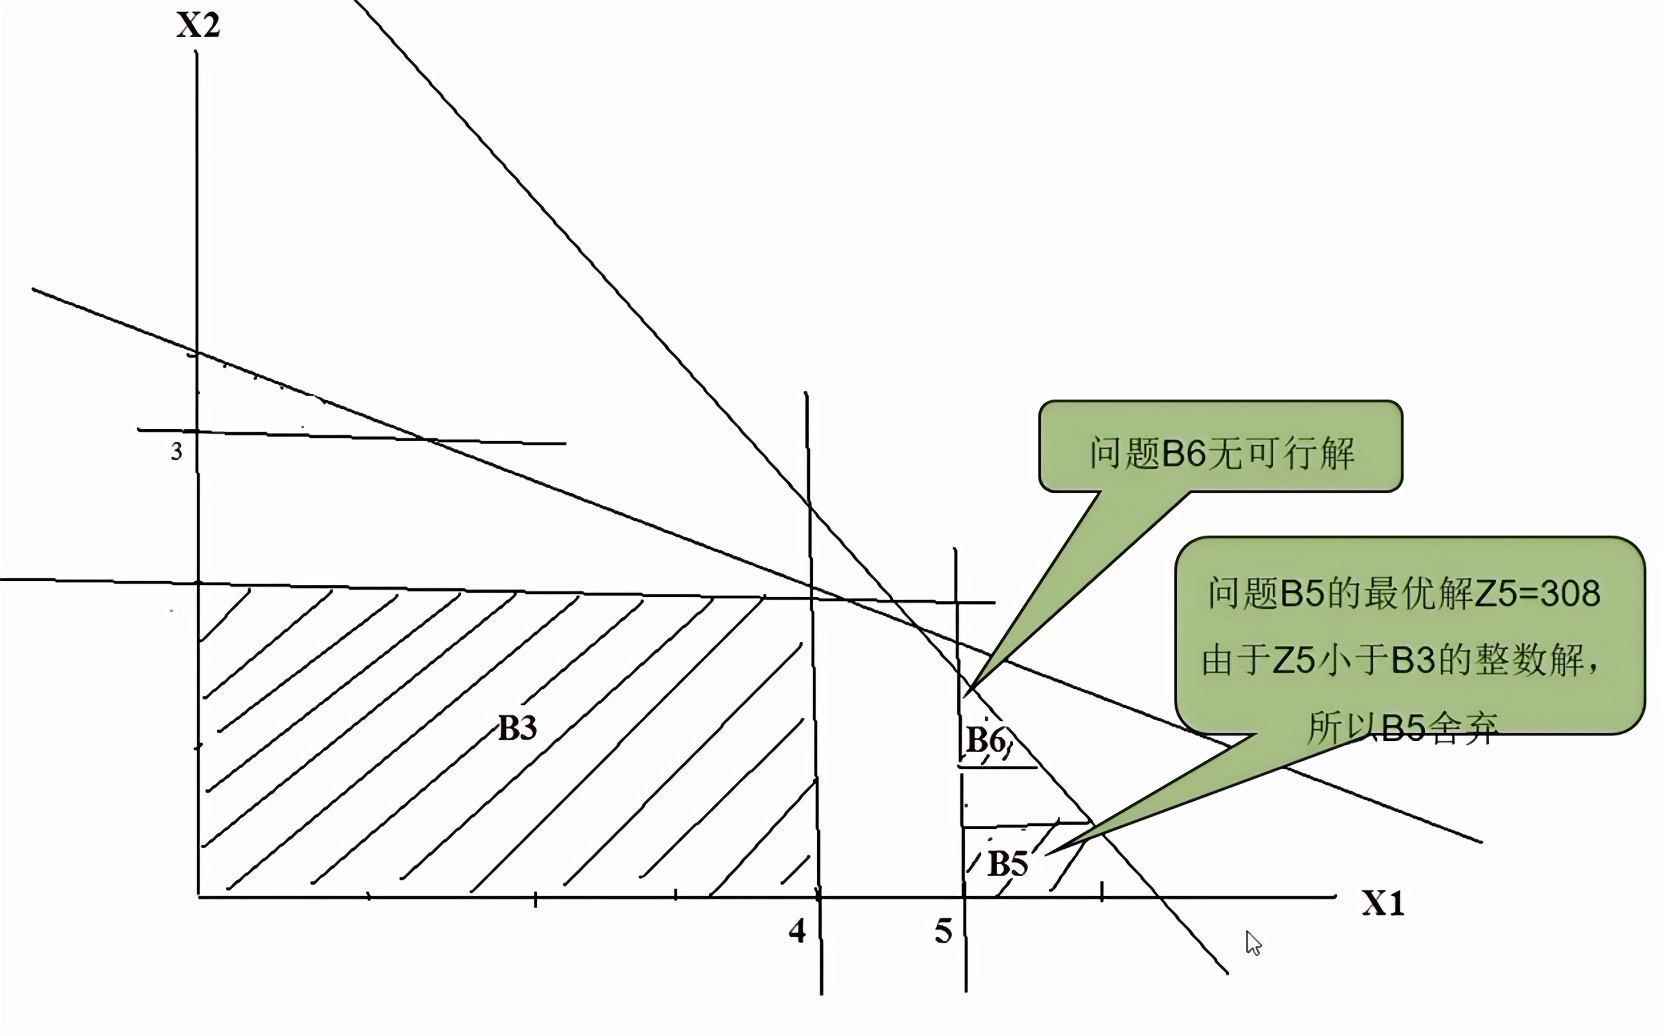
\includegraphics[width=0.8\textwidth]{./image/14.png}
            \caption{第三次迭代}
            \label{fig:Chapter4_Temporary_Pavilion_4}
        \end{figure}

        \end{exbox}
        我们不难发现,在上述过程中,除了最开始找了任意一个整数点作为下限,
        其他的计算过程全部是\textcolor{red}{线性规划}的过程。即过程分为两类:
        \begin{itemize}
            \item (计算过程)线性规划求解:即求解B问题的最优解。
            \item (判断过程)分枝:即对B问题进行分割,得到子区域B1、B2、B3、B4等。同时进行判断并更新上限和下限。
        \end{itemize}
        实际上我们在做的,就是先算B问题的最优解,如果需要则进行分割,再分别算子区域的最优解。并依据子区域更新上限和下限。实际上是取各个子区域上下限的交集。
        \begin{itemize}
            \item 如果发现子区域最优值小于等于当前下限,则该子区域没有继续分割的必要了。
            \item 如果发现子区域最优值小于当前上限,则应该更新上限。
            \item 如果上下限互相逼近到相等,问题可以结束。即证明某一子区域整数最优解所对应的最优值比其他子区域的都要大。
        \end{itemize}
        \begin{notebox}{\textbf{分枝定界法的要点}}
            \begin{itemize}
                \item \textbf{分枝}:分为多个更小的空间
                \item \textbf{定界}:确定每个小空间的上、下限和总的上、下界
                \item \textbf{剪枝}:据每个小空间的上、下限和总的上、下界,删掉那些明显\textcolor{red}{低于总下界}和\textcolor{red}{无可行解}的小空间。
            \end{itemize}
        \end{notebox}
        \begin{figure}[H]
            \centering
            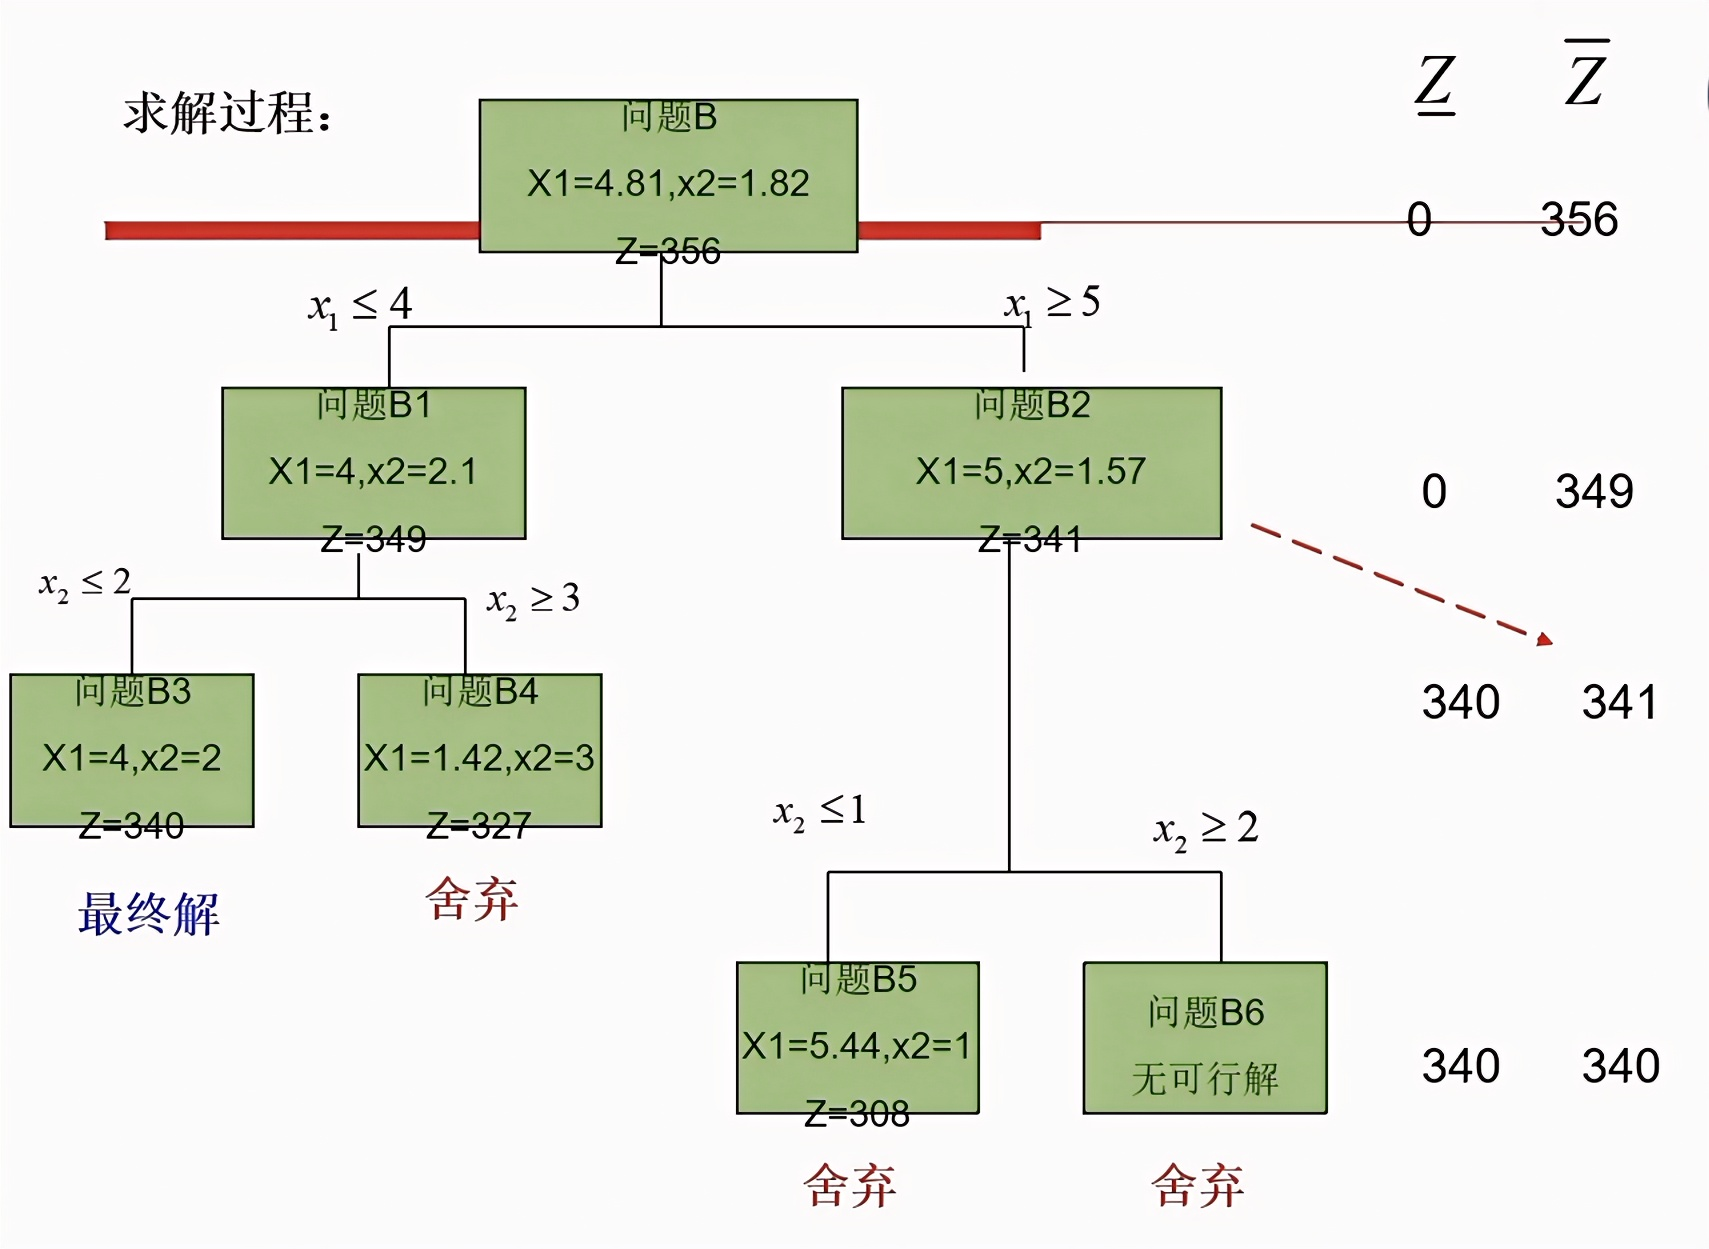
\includegraphics[width=0.8\textwidth]{./image/15.png}
            \caption{例题总体思路}
            \label{fig:Chapter4_Temporary_Pavilion_4}
        \end{figure}
    
    \section{0-1规划及其求解方法}
    \subsection{0-1规划的定义和数学模型}
    \begin{dfnbox}{0-1规划}{amznotes}
        如果整数规划问题中的所有决策变量 $x_i$,$(i=1, 2, \cdots, n)$ 仅限于取 0 或 1 两个值,则称此问题为 0-1 整数规划,简称为\textbf{0-1 规划},其变量 $x_i$,$(i=1, 2, \cdots, n)$ 称为\textbf{0-1 变量},或\textbf{二进制变量},相应的决策变量取值的约束为 $x_i = 0$ 或 1,等价于 $x_i \geq 0$ 且 $x_i \leq 1$,且为整数。
    \end{dfnbox}
    \begin{dfnbox}{0-1混合整数规划}{amznotes}
        如果整数规划问题中的一部分决策变量为 0-1 变量,则称为 \textbf{0-1 混合整数规划}。
    \end{dfnbox}
    0-1 规划可以是线性的,也可以是非线性的,0-1 整数规划的一般模型为:
    \begin{thmbox}{0-1 整数规划的一般模型}{cool}
        \begin{center}
            \begin{equation*}
            \max \quad (\min) \quad z = \sum_{j=1}^n c_j x_j
            \end{equation*}
            \begin{equation*}
            \text{s.t.} \quad \sum_{j=1}^n a_{ij} x_j \leq (\text{或 } =, \geq) \, b_i \quad (i=1, 2, \cdots, m),
            \end{equation*}
            \begin{equation*}
            x_j = 0 \text{ 或 } 1 \quad (j=1, 2, \cdots, n).
            \end{equation*}
            \end{center}
    \end{thmbox}

    \subsection{0-1规划的例题}
    \begin{exbox}{\textbf{销售网点问题}}
    1\textbf{例:} 某公司拟在城东、城西、城南新建销售网点,有 7 个位置 A1, A2, A3, A4, A5, A6, A7 可选。考虑组建成本和总体布局,规定:

    \textbf{城东:} A1, A2, A3 中至多选择 2 个

    \textbf{城西:} A4, A5 中至少选择 1 个

    \textbf{城南:} A6, A7 至少选择 1 个

    若选 $A_i$,则建设投资为 $b_i$,预计获利 $c_i$,但投资总额不能超过 $B$ 元。如何选择址获利最大?
    \\
    \textbf{解:} 设决策变量 $x_i(i=1,2\cdots 7)$

    \begin{center}
    \begin{equation*}
    x_i = 
    \begin{cases} 
    1 & \text{A}_i \text{被选中}, \quad i=1,2\cdots 7 \\
    0 & \text{A}_i \text{未选中}
    \end{cases}
    \end{equation*}
    \end{center}

    则

    \begin{align*}
    \max \quad z &= \sum_{i=1}^7 c_i x_i \\
    \text{s.t.} \quad & \sum_{i=1}^7 b_i x_i \leq B \\
    & x_1 + x_2 + x_3 \geq 2 \\
    & x_4 + x_5 \geq 1 \\
    & x_6 + x_7 \geq 1 \\
    & x_i = 0,1, \quad i=1,2\cdots 7
    \end{align*}

    为 0-1 规划。
    \end{exbox}

    \begin{exbox}{\textbf{一般的指派问题(分派问题)}}
        1\textbf{例:} 在实际生产管理中,总希望把有限的资源(人员、资金等)最佳地指派,以发挥其最高的工作效率,创造最大的价值。
        例如,某科研部门有n项任务,正好需要n个人去完成,由于任务的性质和每个人的专长不同,每个人完成各项任务的效率(时间或成本)如表4.2所示。如果指派每个人仅能完成一项任务,每项任务仅要一个人去完成,如何分派使完成这n项任务的总效率(效益量化)为最高,这是典型的标准指派问题。
        \begin{table}[H]
            \centering
            \label{tab:4-2}
            \renewcommand{\arraystretch}{1.5}
            \begin{tabular}{|c|c|c|c|c|}
                \hline
                人$\backslash$项 & 1 & 2 & $\cdots$ & n \\
                \hline
                1 & $c_{11}$ & $c_{12}$ & $\cdots$ & $c_{1n}$ \\
                \hline
                2 & $c_{21}$ & $c_{22}$ & $\cdots$ & $c_{2n}$ \\
                \hline
                $\vdots$ & $\vdots$ & $\vdots$ & $\ddots$ & $\vdots$ \\
                \hline
                n & $c_{n1}$ & $c_{n2}$ & $\cdots$ & $c_{nn}$ \\
                \hline
            \end{tabular}
            \caption{指派问题的利润元成表矩阵}
        \end{table}
        
        \textbf{解:} 设指派问题的效益矩阵为 $(c_{ij})_{n \times n}$,其元素 $c_{ij}$ 表示指派第 $i$ 个人去完成第 $j$ 项任务时所获得的效益($>0$)。或者说:以 $c_{ij}$ 表示指派给 $i$ 的第 $j$ 单位资源分配用于第 $j$ 项任务时的有关效益。设问题的决策变量为 $x_{ij}$,是 0-1 变量,即
        
        \begin{center}
        \begin{equation*}
        x_{ij} = 
        \begin{cases} 
        1, & \text{当指派第 $i$ 个人去完成第 $j$ 项任务时}, \\
        0, & \text{当下指派第 $i$ 个人去完成第 $j$ 项任务时}.
        \end{cases}
        \end{equation*}
        \end{center}
        
        则其数学模型为
        
        \begin{align*}
        &\max (\min) \quad z = \sum_{i=1}^n \sum_{j=1}^n c_{ij} x_{ij} \\
        \text{s.t.} \quad & \sum_{j=1}^n x_{ij} = 1 \quad (i=1, 2, \cdots, n), \tag*{第 $i$ 个人做成一项任务} \\
        & \sum_{i=1}^n x_{ij} = 1 \quad (j=1, 2, \cdots, n), \tag*{第 $j$ 项任务只能由一个人完成} \\
        & x_{ij} = 0 \text{ 或 } 1 \quad (i, j=1, 2, \cdots, n).
        \end{align*}
        \end{exbox}

    \subsection{0-1规划的求解}
    \begin{dfnbox}{显枚举法}{amznotes}
        显枚举法(又称为穷举法)是把所有可能的组合情况(共2n种组合)列举出后进行比较,找到所需要的解。这种方法对于变量个数较多时,易产生“组合爆炸”,计算量非常巨大。
    \end{dfnbox}
    \begin{dfnbox}{隐枚举法}{amznotes}
        隐枚举法是从实际出发,从所有可能的组合取值中利用过滤条件排除些不可能是最优解的情况,只需考查一部分的组合就可以得到最优解。因此,隐枚举法又称为部分枚举法。
    \end{dfnbox}
    \begin{exbox}{隐枚举求解}
        1\textbf{例:} 用隐枚举求解
        \[
        \max \quad z = 3x_1 - 2x_2 + 5x_3
        \]

        \[
        \begin{array}{r@{\,}c@{\,}l}
        x_1 + 2x_2 - 3x_3 & \leq & 2 \quad (1) \\
        x_1 + 4x_2 + x_3 & \leq & 4 \quad (2) \\
        x_1 + x_2 & \leq & 3 \quad (3) \\
        4x_2 + x_3 & \leq & 6 \quad (4) \\
        x_1, x_2, x_3 & = & 0, 1 \quad (5)
        \end{array}
        \]

        \textbf{解:} 对于三变量的0-1规划, 所有变量组合为

        \[
        \begin{array}{c@{\,}c@{\,}c@{\,}c@{\,}c@{\,}c@{\,}c@{\,}c@{\,}c@{\,}c}
        (0,0,0), & (0,0,1), & (0,1,0), & (0,1,1), & (1,0,0), & (1,0,1), & (1,1,0), & (1,1,1).
        \end{array}
        \]

        首先, 通过试探方法找一个可行解, 例如 (1,0,0) 就是满足所有约束条件的可行解之一, 计算 $z(1,0,0)=3$\\

        对于上述极大化0-1规划, 其最优值$z*$当然大于等于这个初始的任意解$z(1,0,0)$, 所以有
        \[
        z = 3x_1 - 2x_2 + 5x_3 \geq 3 \quad (6)
        \]

        可以想象, 如果以 (6) 来进一步约束原问题A, 则那些$z<3$的变量组合就可以直接舍弃。换句话说, 后边只要检查$z>=3$的变量组合就能确定最优解——这就是 “取0-1变量组合的一部分” 的含义。

        然后, 把 (6) 标为约束条件, 作为一个新的约束条件加入到原问题A:

        \[
        \max \quad z = 3x_1 - 2x_2 + 5x_3
        \]

        \[
        \begin{array}{r@{\,}c@{\,}l}
        x_1 + 2x_2 - 3x_3 & \leq & 2 \quad (1) \\
        x_1 + 4x_2 + x_3 & \leq & 4 \quad (2) \\
        x_1 + x_2 & \leq & 3 \quad (3) \\
        4x_2 + x_3 & \leq & 6 \quad (4) \\
        3x_1 - 2x_2 + 5x_3 & \geq & 3 \quad (6) \\
        x_1, x_2, x_3 & = & 0, 1 \quad (5)
        \end{array}
        \]
        新问题等价于原问题。
        构造0-1规划约束条件检查表\footnote{对科幻感兴趣的同学,不妨把这几个约束条件分别视为文明发展中的“大过滤器”,这将有助于理解。对于活到宇宙最后的那些“文明”,再去比比谁发展的好吧! }将所有约束条件按(6)(1)(2)(3)(4)顺序排好,对每个解依次代入每个约束条件左侧,求出数值,看是否满足约束条件。如果某一约束条件不满足,同一行以下各约束条件就不再检查,因而减少了运算次数。
        \begin{figure}[H]
            \centering
            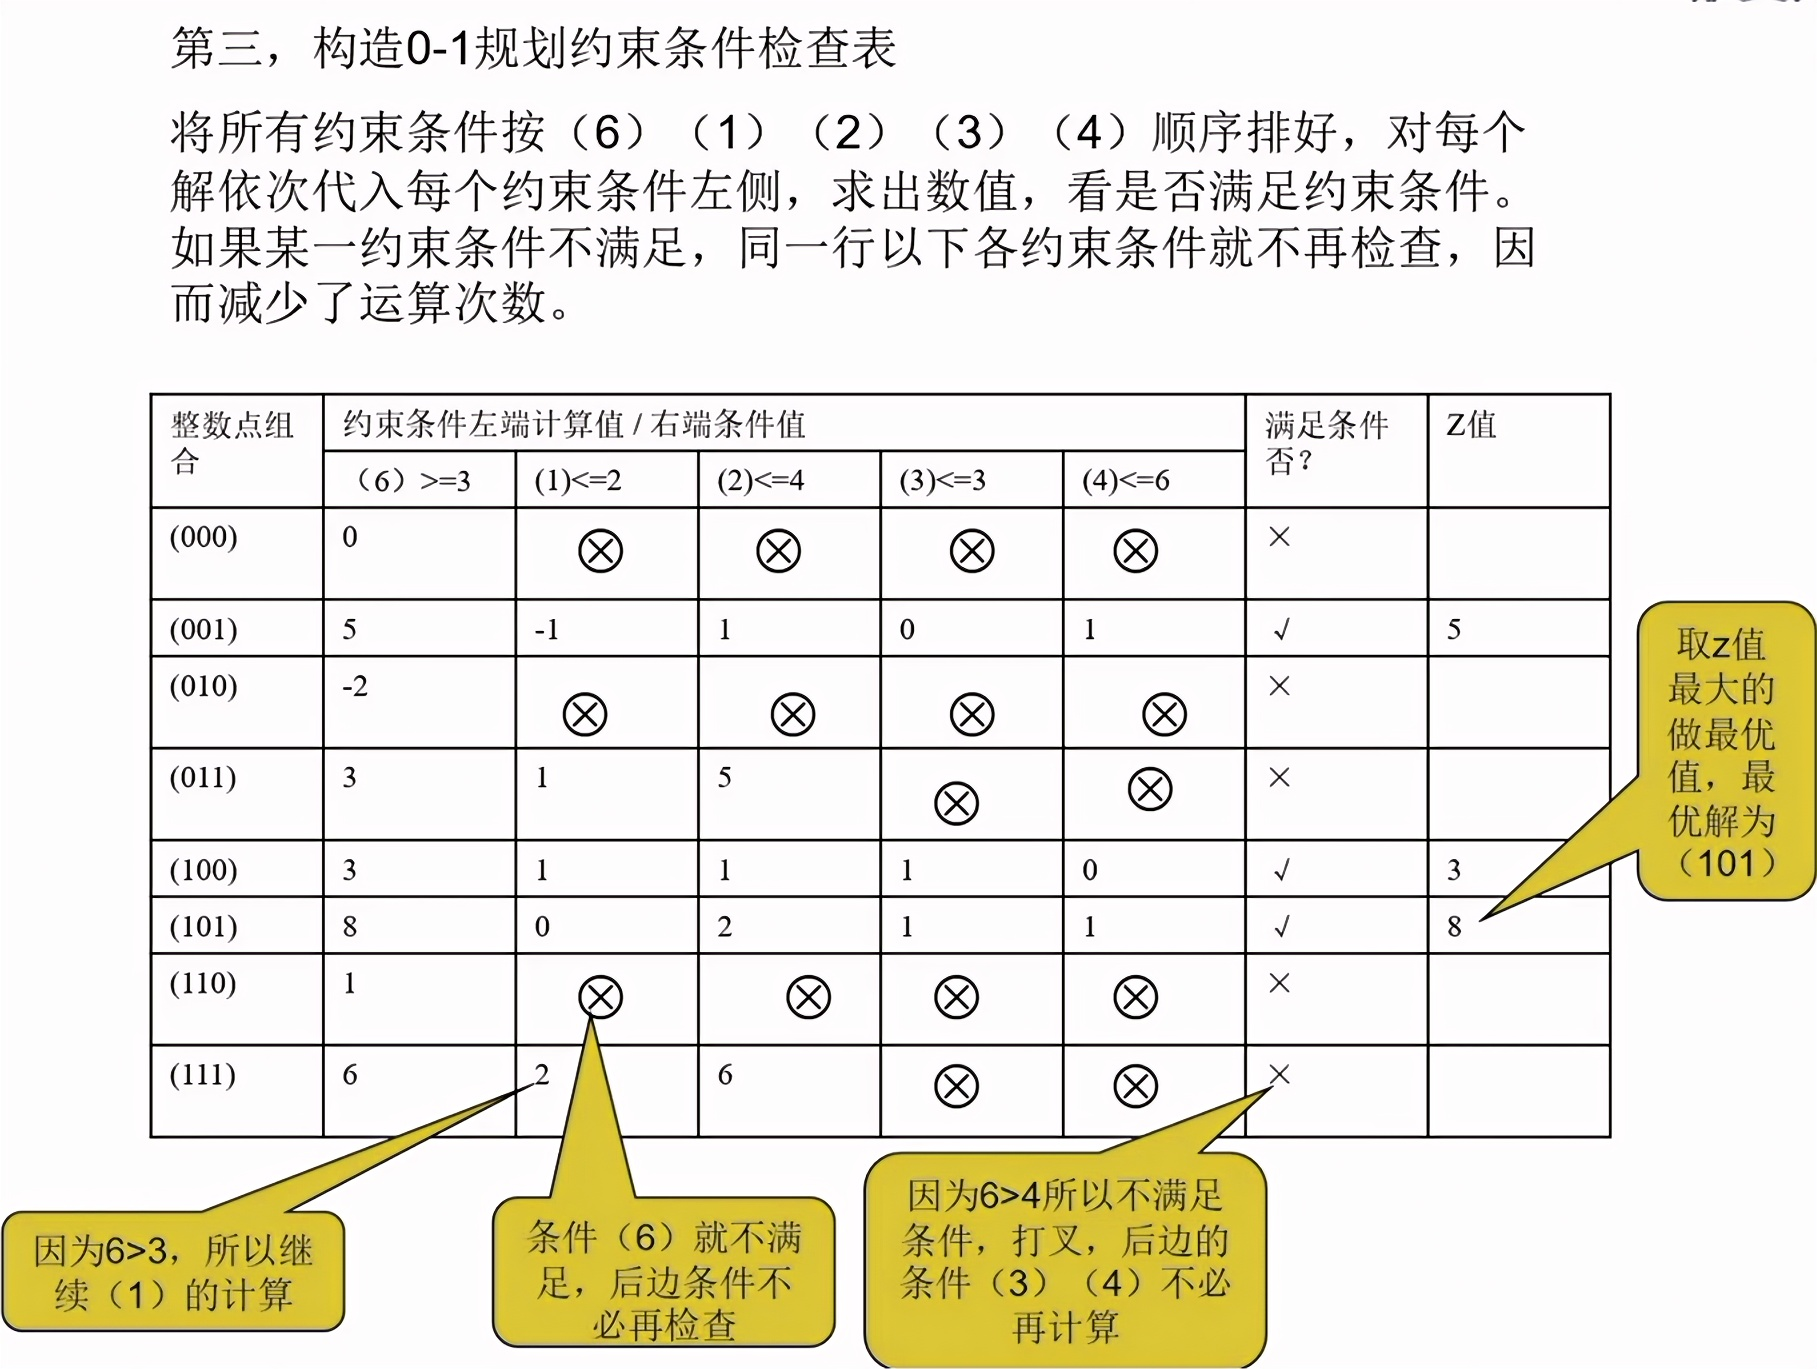
\includegraphics[width=0.8\textwidth]{./image/16.png}
            \caption{0-1规划约束条件检查表}
            \label{fig:Chapter4_Temporary_Pavilion_1}
        \end{figure}
    \end{exbox}







    \section{案例分析}
    \begin{exbox}{\textbf{生产计划问题}}
    1\textbf{例:}某工厂配套生产某种专业电子产品,今年前6个月收到的该产品的订货数量分别为 3000件,4500件,3500件,4000件,4000件和5000 件.已知该厂的正常生产能力为每月 3000件,利用加班生产还可以生产 1500 件.正常生产的成本为每件 5000 元,加班生产还要增加1500 元的成本,库存成本为每件每月200元.试问该厂如何组织安排生产才能在保证完成生产计划的情况下使生产成本最低?
    \textbf{解:} 根据这个问题的实际情况,设$x_i$表示第$i$个月正常生产的产品数量;
    $y_i$表示第$i$个月加班生产的产品数量;$z_i$表示第$i$个月月初产品的库存数量。
    $d_i$表示第$i$个月的需求量$(i=1,2,\cdots,6)$,并且第1个月月初的库存为 0,则问题的生产成本为:
    $$
        \sum_{i=1}^{6}(5000x_i+6500y_i+200z_i)
    $$
    三项分别为正常生产成本、加班生产成本和库存成本。
    \end{exbox}
    \begin{exbox}{\textbf{游泳队员分配问题}}
        1\textbf{例:}某游泳队拟选用 A,B,C,D 四名游泳运动员组成一个 4x100m 混合泳接力队,参加大型运动会,他们的100m自由泳,蛙泳,蝶泳,仰泳的成绩如下表 4.3 所示.A,B,C,D 四名运动员各自游什么姿势,才最有可能取得最好成绩?
        \begin{table}[H]
            \centering
            \label{tab:4.3}
            \renewcommand{\arraystretch}{1.5}
            \begin{tabular}{|c|c|c|c|c|}
                \hline
                & 自由泳 & 蝶泳 & 蛙泳 & 仰泳 \\ \hline
                A & 56 & 74 & 61 & 63 \\ \hline
                B & 63 & 69 & 65 & 71 \\ \hline
                C & 57 & 77 & 63 & 67 \\ \hline
                D & 55 & 76 & 62 & 62 \\ \hline
            \end{tabular}
            \caption{队员的游泳成绩}
        \end{table}
        \textbf{解:} 根据题意,假设问题的决策变量为 $x_{ij}$,令 $i$ 名队员游泳第 $j$ 种姿势,$x_{ij}$ 的取值如下:
        \[
        x_{ij} =
        \begin{cases}
        1, & \text{让} i \text{名队员游泳第} j \text{种姿势,} \\
        0, & \text{不让} i \text{名队员游泳第} j \text{种姿势.}
        \end{cases}
        \]
        其中 $i=1,2,3,4$ 分别表示自由泳、蛙泳、蝶泳、仰泳。根据问题的要求可知,四名运动员的成绩矩阵为

        \[
        A = \left( a_{y} \right)_{4 \times 4} =
        \begin{pmatrix}
        56 & 74 & 61 & 63 \\
        63 & 69 & 65 & 71 \\
        57 & 77 & 63 & 67 \\
        55 & 76 & 62 & 62
        \end{pmatrix}
        \]
        以 $4 \times 100m$ 混合泳所用的总时间最小为目标,以每名运动员游一个项目,每一个项目只能有一名运动员完成为约束,这是一个标准的分派问题。$4 \times 100m$ 混合泳所用的总时间为:

        \[
        T = \sum_{i=1}^4 \sum_{j=1}^4 a_{y} x_{ij}
        \]
        该模型为一个 $0-1$ 整数规划模型。

        \begin{align*}
            \text{min } T &= \sum_{i=1}^4 \sum_{j=1}^4 a_{y} x_{ij} \\
            \text{s.t.} \quad & \left\{
            \begin{aligned}
            \sum_{i=1}^4 x_{ij} &= 1, \quad (j=1,2,3,4) \\
            \sum_{j=1}^4 x_{ij} &= 1, \quad (i=1,2,3,4) \\
            x_{ij} &= 0 \text{ 或 } 1, \quad (i,j=1,2,3,4)
            \end{aligned}
            \right.
        \end{align*}

    \end{exbox}
\ifx\allfiles\undefined
	
	% 如果有这一部分的参考文献的话,在这里加上
	% 没有的话不需要
	% 因此各个部分的参考文献可以分开放置
	% 也可以统一放在主文件末尾。
	
	%  bibfile.bib是放置参考文献的文件,可以用zotero导出。
	% \bibliography{bibfile}
	
	end{document}
	\else
	\fi